\documentclass[letterpaper, reqno,11pt]{article}
\usepackage[margin=1.0in]{geometry}
\usepackage{color,latexsym,amsmath,amssymb,graphicx,float,listings,tikz}
\usepackage{hyperref}

\hypersetup{
colorlinks=true,
linkcolor=magenta,
filecolor=magenta,
urlcolor=cyan,
}

\graphicspath{ {images/} }

\begin{document}
\pagenumbering{arabic}
\title{Math 443 Homework 6}
\date{15/03/23}
\author{Xander Naumenko}
\maketitle

\tikzstyle{vertex}=[shape=circle, minimum size=2mm, fill, draw, inner sep=0]

{\medskip\noindent\bf Question 1a.} See below, $x,y$ are a minimum separating set and clearly $x,y$ are adjacent to both $u$ and $v$. 

\begin{center}
\begin{tikzpicture}
\draw (0,1)node[label=u,vertex]{};
\draw (1,0)node[label=x,vertex]{};
\draw (1,2)node[label=y,vertex]{};
\draw (2,1)node[label=v,vertex]{};
\draw (0,1)--(1,0);
\draw (0,1)--(1,2);
\draw (2,1)--(1,2);
\draw (2,1)--(1,0);
\end{tikzpicture}
\end{center}

{\medskip\noindent\bf Question 1b.} $x,y$ is a minimum separating set with the required properties. 

\begin{center}
\begin{tikzpicture}
\draw (0,1)node[label=u,vertex]{};
\draw (1,0)node[label=x,vertex]{};
\draw (1,2)node[vertex]{};
\draw (2,0)node[vertex]{};
\draw (2,2)node[label=y,vertex]{};
\draw (3,1)node[label=v,vertex]{};
\draw (0,1)--(1,0);
\draw (0,1)--(1,2);
\draw (1,2)--(2,2);
\draw (1,0)--(2,0);
\draw (3,1)--(2,2);
\draw (3,1)--(2,0);
\end{tikzpicture}
\end{center}

{\medskip\noindent\bf Question 1c.} The following graph works. Here I have listed a particular $x,y$, but once you choose one member of the separating set to be adjacent to $u$ or $v$ the only other option forces the other vertex adjacent to the same choice of $u,v$. 

\begin{center}
\begin{tikzpicture}
\draw (0,1)node[label=u,vertex]{};
\draw (1,0)node[label=x,vertex]{};
\draw (1,2)node[label=y,vertex]{};
\draw (2,0)node[vertex]{};
\draw (2,2)node[vertex]{};
\draw (3,1)node[label=v,vertex]{};
\draw (0,1)--(1,0);
\draw (0,1)--(1,2);
\draw (1,2)--(2,2);
\draw (1,0)--(2,0);
\draw (1,2)--(2,0);
\draw (1,0)--(2,2);
\draw (3,1)--(2,2);
\draw (3,1)--(2,0);
\end{tikzpicture}
\end{center}

{\medskip\noindent\bf Question 2.} By Menger's Theorem it suffices to provide an upper bound on $\kappa(u,v)$ and a lower bound on $\lambda(u,v)$, as long as they're the same then the two graphs must be equal. In figure \ref{fig:2a} I give an example of a degree $5$ $u-v$ separating set and in figure \ref{fig:2b} I give an example of 5 disjoint paths between $u$ and $v$, so by Menger's Theorem $5\geq \kappa(u,v)=\lambda(u,v)\geq 5\implies \lambda(u,v)=5$. $\square$

\begin{figure}[htpb]
    \centering
    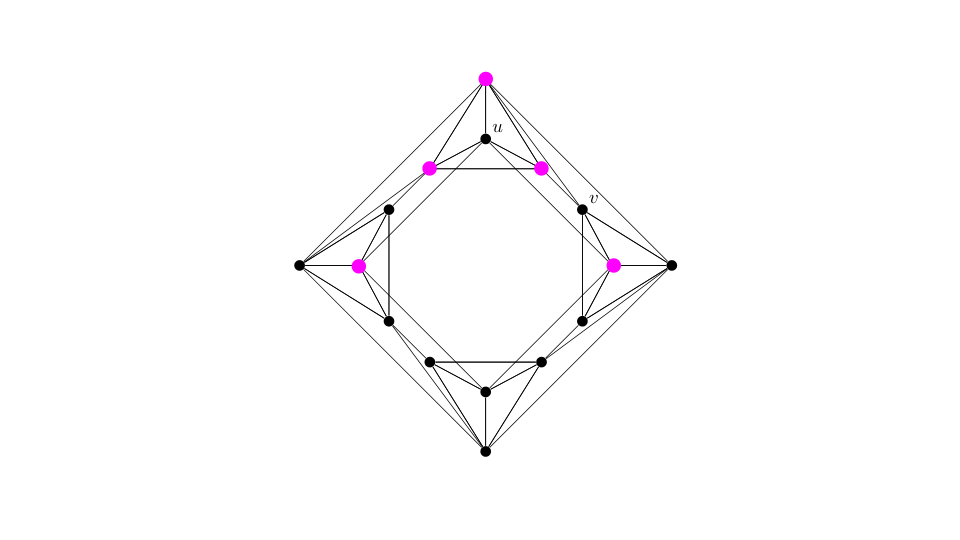
\includegraphics[width=0.8\textwidth]{2a}
    \caption{Graph for 2 with a $u-v$ separating set.}
    \label{fig:2a}
\end{figure}

\begin{figure}[htpb]
    \centering
    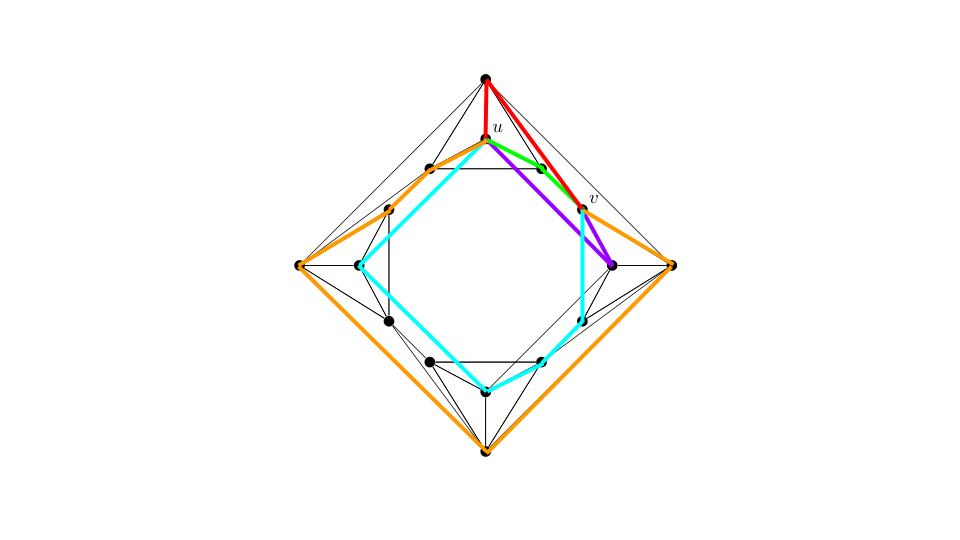
\includegraphics[width=0.8\textwidth]{2b}
    \caption{Graph for 2 with disjoint $u-v$ paths.}
    \label{fig:2b}
\end{figure}

{\medskip\noindent\bf Question 3.} Consider a new graph $G'$ that is a copy of $G$ with an additional vertex $v$ that is adjacent to each of the $v_i$. I claim that $G'$ is $k$-connected. Let $x,y\in V(G')$. If $x$ and $y$ are both in $G$ then a vertex set of size less than $k$ clearly can't separate them due to the $k$-connectivity of $G$, so assume $y=v$. Let $S\subset V(G)$ be a set of vertices on $G'-x-v$ with $|S|<k$. $G$ is $k$-connected so there still exists a path from $x$ to $v_i$ in $G-S$ for all $v_i$ that are in $G-S$. $|S|<k$ so at least on such $v_i$ is still in $G'-S$, so there exists a path from $x$ to $v_i$ and an edge from $v_i$ to $v$, so $v$ and $x$ are connected in $G'-S$. Thus $G'$ is $k$-connected. 

Now apply Menger's Theorem to $u$ and $v$ on $G'$. $G'$ is $k$-connected as justified above, so $\kappa(u,v)\geq k\implies \lambda(u,v)\geq k$ (although by our construction we know equality holds, it's not important). Let $P_1', \ldots, P_k'$ be $k$ disjoint paths from $u$ to $v$ which are guaranteed to exist by our bound of $\lambda$. The only neighbors of $v$ for the $k$ paths to go through are each of the $v_i$ of which there are $k$, so each path must go through exactly one. Letting $P_i=P_i'-v$, these now fill the requirements of the $P_i$ asked for in the question and we're done. $\square$

{\medskip\noindent\bf Question 4.} Clearly $\kappa(G_r)\leq \kappa(G)+r$, since you can take a separating set of $G$ and remove all $r$ new vertices to separate $G_r$. To show that this is also an lower bound, let $S$ be a vertex set with $|S|<\kappa(G)+r$. Let $u,v\in G_r$. If any of the $r$ new vertices are in $G_r-S$, then $u$ and $v$ are both connected to that vertex (or are that vertex), so they are connected. Therefore $G_r-S\subset G$. 

It takes $r$ vertices of $S$ to remove all the $r$ new vertices, so $S$ contains less than $\kappa(G)$ vertices of $G$, so by $\kappa$'s definition $S$ isn't a separating set. Therefore $\kappa(G_r)\geq \kappa(G)+r$, so equality must hold and $\kappa(G_r)=\kappa(G)+r$. $\square$

{\medskip\noindent\bf Question 5.} Both directions will be proven separately. 

($\Rightarrow$) Assume $G$ is $k$-edge-connected, and let $u,v\in V(G)$. By hypothesis a minimum $uv$ separating edge set is of size at least $k$, so the maximum number of pairwise edge-disjoint $uv$ paths is at least $k$ by Theorem 5.21 which is what we needed to prove. 

($\Leftarrow$) Assume that $G$ contains $k$ pairwise edge-disjoint $uv$-paths for each $u,v\in V(G)$. Let $u,v\in V(G)$. The maximum number of pairwise edge-disjoint $uv$ paths in $G$ is always at least $k$, so the maximum number of such paths is greater than or equal to $k$. Thus by Theorem 5.21, a minimum $uv$ separating edge set is of size at least $k$. Since this is true of each $u,v\in V(G)$, $G$ is $k$-edge-connected. $\square$

{\medskip\noindent\bf Question 6.} As the hint suggests we will use strong induction on $k$. 

{\noindent\bf Base case (k=2):} Let $G$ be $2$-connected and let $e_1,e_2\in E(G)$. $G$ contains no cut vertices so by definition it's a block. From homework 5, question 4, all edges in a block share a cycle. Thus $e_1$ and $e_2$ share a cycle in $G$ as required. 

{\noindent\bf Inductive step:} Let $G$ be a $(k+1)$-connected graph, and assume the theorem holds for all graphs of connectivity $k$ or less. Let $e_1,e_2\in E(G)$ and $v_1,\ldots v_{k-1}\in V(G)$. By the inductive hypothesis there exists a cycle $C$ containing $e_1,e_2$ and $v_i\forall i\in [k-2]$. For the simplicity of the proof, extend $C$ with arbitrary other vertices until is has length at least $k+1$. This is possible since $G$ is $k+1$ connected, so we can take two adjacent vertices $x,y, xy\notin \{e_1,e_2\} $ on $C$, and replace the edge between them in $C$ with a path between them on $G-(C-x-y)-xy$. 

By question 3 of this homework (applied to $k+1$ vertices of $C$), there exist $k+1$ disjoint paths from $v_{k-1}$ to $C$ with separate endpoints. For each of these paths, consider the shortened version, starting from its first intersection of $C$, to $v_{k-1}$, call these paths $P_i,i\in [k+1]$. Since the paths are disjoint their endpoints in $C$ are also still distinct. 

Let $S=(v_1,\ldots, e_1, \ldots, e_2,\ldots, v_{k-2})$ be an ordered list of the $v_i$ and $e_1,e_2$ in the order that they occur in $C$ (the indices on the $v_i$s were arbitrary, so we can rename so that they are in order). Since there are $k$ elements of $S$ and $k+1$ paths ending on $C$ on distinct vertices, by the pidgeonhole principle it must be that there are elements of $S$, $s_1$ and $s_2$ that are adjacent such that two paths $P_i$ and $P_j$ have endpoints $u_i$, $u_j$ between them in $C$. The awkwardness of the wording comes from the fact that $s_1$ and $s_2$ could be either edges or vertices, what I mean by between is that the subpath of $C$ between $u_i$ and $u_j$ does not contain $s_1$ or $s_2$ as neither edges nor inner vertices (although if $s_1$ or $s_2$ are a vertex it could be that for example $u_i=s_1$). Thus we can extend $C$ by considering the new cycle $C'=u_iP_iv_{k-1}P_ju_jCu_i$, and by our choice of $u_i,u_j$ this cycle contains both $e_1,e_2$ as well as all the $v$s. $\square$

%Assign $C$ an direction. Let $u_1$ be the endpoint of $e_1$ later in $C$ according to its direction, while let $u_2$ be the endpoint of $e_2$ earlier in $C$. 

{\medskip\noindent\bf Question 7.} $\square$ (pretty concise proof, huh)

%Let $G=\{v_i: i\in [n]\} $ be a $k$-connected, $r$-regular graph such that $\forall i\in V(G),\exists m\in [n]$ s.t. $v_i,v_{i+1},\ldots,v_{i+m}\subset K_{r,2}$. I don't actually have to prove anything about $G$ since there's no question, so we're done. $\square$

{\medskip\noindent\bf Question 8.} Let $c$ be a circuit in a graph $G$ with ordered vertices $v_1,v_2,\ldots,v_n$ (potentially some repeats). Let $v_j$ be the first repeated vertex (i.e. minimal $j$), and let $i$ be the index of the vertex that $v_j$ first occurred in. Then $v_i, v_{i+1}, \ldots, v_j$ is a closed walk with no repeated vertices by the minimally of $j$ which is exactly the definition of a cycle so we're done. $\square$

\end{document}
